\documentclass{article}

%-----------------------------------------------------------------------------
%	Packages
%-----------------------------------------------------------------------------
\usepackage[utf8]{inputenc}	% für Umlaute ect.
\usepackage{fancyhdr} % für header
\usepackage{lastpage} % für footer
\usepackage{extramarks} % für header und footer
\usepackage{amsthm} % math stuff
\usepackage{amsmath} % math stuff
\usepackage{amssymb} % math stuff
\usepackage{color}
\usepackage{listings} % code listings
\usepackage{enumitem}
\usepackage{graphicx} % für graphics
\usepackage{hyperref}
\usepackage{caption}
\usepackage{subcaption}
\usepackage{multicol}
\usepackage{pgf}
\usepackage{tikz}
\usetikzlibrary{arrows,automata} 

%-----------------------------------------------------------------------------
%	Allegmeine Dokumentsettings
%-----------------------------------------------------------------------------
% Margins
\topmargin=-0.45in
\evensidemargin=0in
\oddsidemargin=0in
\textwidth=6.5in
\textheight=9.0in
\headsep=0.25in
%Header und Footer
\pagestyle{fancy}
\chead{\moduleTitle}  
\rhead{}
\lfoot{\lastxmark}
\cfoot{} 
\rfoot{\ \thepage\ of\ \protect\pageref{LastPage}}
\renewcommand\headrulewidth{0.4pt} % Size of the header rule
\renewcommand\footrulewidth{0.4pt} % Size of the footer rule

% Zeilenabstand
\linespread{1.0} 

%----------------------------------------------------------------------------------------
%	Commands and Environments
%----------------------------------------------------------------------------------------

%---- Allows vertical lines in matrices
\makeatletter
\renewcommand*\env@matrix[1][*\c@MaxMatrixCols c]{%
	\hskip -\arraycolsep
	\let\@ifnextchar\new@ifnextchar
	\array{#1}}
\makeatother
%--------------------------

\newcommand{\moduleTitle}{Projektarbeit - Graphische Modelle}
\newcommand{\moduleSubTitle}{Theoretische Informatík I}
\newcommand{\moduleClassInstructor}{Prof. Joachim Giesen}
\newcommand{\university}{FSU Jena}
\newcommand{\moduleSemester}{SS 17}
\newcommand{\authorName}{Matthias Mitterreiter}

% Für Code listings
\lstset{ %
	language=Python,                % choose the language of the code
	basicstyle=\footnotesize,       % the size of the fonts that are used for the code
	numbers=left,                   % where to put the line-numbers
	numberstyle=\footnotesize,      % the size of the fonts that are used for the line-numbers
	stepnumber=1,                   % the step between two line-numbers. If it is 1 each line will be numbered
	numbersep=5pt,                  % how far the line-numbers are from the code
	backgroundcolor=\color{white},  % choose the background color. You must add \usepackage{color}
	showspaces=false,               % show spaces adding particular underscores
	showstringspaces=false,         % underline spaces within strings
	showtabs=false,                 % show tabs within strings adding particular underscores
	frame=single,           % adds a frame around the code
	tabsize=2,          % sets default tabsize to 2 spaces
	captionpos=b,           % sets the caption-position to bottom
	breaklines=true,        % sets automatic line breaking
	breakatwhitespace=false,    % sets if automatic breaks should only happen at whitespacee
	escapeinside={\%*}{*)}          % if you want to add a comment within your code
}

% An environment for stpes, cases ect. 
% From: http://tex.stackexchange.com/questions/32798/a-step-by-step-environment
	\newenvironment{steps}[1]{\begin{enumerate}[label=#1 \arabic*]}{\end{enumerate}}
\makeatletter%
\def\step{%
	\@ifnextchar[ \@step{\@noitemargtrue\@step[\@itemlabel]}}
\def\@step[#1]{\item[#1]\mbox{}\\\hspace*{\dimexpr-\labelwidth-\labelsep}}
\makeatother

%http://tex.stackexchange.com/questions/10669/how-to-enumerate-equations
\def\Item$#1${\item $\displaystyle#1$
   \hfill\refstepcounter{equation}(\theequation)}

%-----------------------------------------------------------------------------
%	Theoreme
%-----------------------------------------------------------------------------
\theoremstyle{definition}
\newtheorem{mydef}{Definition}
\newtheorem*{mydef*}{Definition}
\newtheorem{mybei}{Beispiel}
\newtheorem*{mybei*}{Beispiel}\begin{frame}
	\frametitle{Aufgabenbeschreibung}
	\framesubtitle{Aufgabenbeschreibung - Evaluate}
	\setbeamertemplate{enumerate items}[default]
	
	\begin{flalign*}
	\left(\begin{array}{cccc}
	\tikzmarkin[ver=style cyan]{col 1}\x  & \x  & \tikzmarkin[ver=style green]{col 2} \x & \x \\
	0   & \x  & \x & \x \\
	0   & 0   & \x & \x \\
	0   & 0   & 0  & \x \\
	a \tikzmarkend{col 1}  &  b  &  c  \tikzmarkend{col 2} &  d \\
	\end{array}\right)
	\end{flalign*}
	\begin{flalign*}
	\begin{pmatrix}
	\Delta z \\
	\Delta y
	\end{pmatrix}
	= 
	\begin{pmatrix}
	a \\
	b
	\end{pmatrix}
	+
	\begin{pmatrix}
	Z & L \\
	J & Y 
	\end{pmatrix}
	\times
	\begin{pmatrix}
	\Delta x \\
	|\Delta z |
	\end{pmatrix}
	\end{flalign*}
	\begin{flalign*}
	\left(\begin{array}{c}
	\Delta z_1 \\
	\vdots \\
	\Delta z_s \\
	\Delta y_1 \\
	\vdots \\
	\Delta y_m
	\end{array}\right)  =
	\left(\begin{array}{c}
	a_1 \\
	\vdots \\
	a_s \\
	b_1 \\
	\vdots \\
	b_m \\
	\end{array}\right) +
	\left(\begin{array}{cccccc}
	Z_{1,1} & \dots & Z_{1,n} & 0 & \dots  & 0 \\
	\vdots & \ddots & \vdots  & L_x & \ddots & 0 \\
	Z_{s,1} & \dots & Z_{s,n} & L_x & L_x & 0 \\
	J_{1,1} & \dots & J_{1,n} & Y_{1,1} & \dots & Y_{1,s} \\
	\vdots  & \ddots & \vdots & \vdots & \ddots & \vdots \\
	J_{m,1} & \dots  & J_{m,n} & Y_{m,1} & \dots & Y_{m,s} \\
	\end{array}\right) \times
	\left(\begin{array}{c}
	\Delta x_1 \\
	\vdots \\
	\Delta x_n \\
	|\Delta z_1 | \\
	\vdots \\
	| \Delta z_s| \\
	\end{array}\right)
	\end{flalign*}
	
\end{frame}
%------------------------------------------------------------------------
\begin{frame}
	\frametitle{Aufgabenbeschreibung}
	\framesubtitle{Aufgabenbeschreibung - Evaluate}
	\setbeamertemplate{enumerate items}[default]
	
	\begin{flalign*}
	\left(\begin{array}{cccc}
	\tikzmarkin[ver=style cyan]{col 1}\x  & \x  & \tikzmarkin[ver=style green]{col 2} \x & \x \\
	0   & \x  & \x & \x \\
	0   & 0   & \x & \x \\
	0   & 0   & 0  & \x \\
	a \tikzmarkend{col 1}  &  b  &  c  \tikzmarkend{col 2} &  d \\
	\end{array}\right)
	\end{flalign*}
	\begin{flalign*}
	\begin{pmatrix}
	\Delta z \\
	\Delta y
	\end{pmatrix}
	= 
	\begin{pmatrix}
	a \\
	b
	\end{pmatrix}
	+
	\begin{pmatrix}
	Z & L \\
	J & Y 
	\end{pmatrix}
	\times
	\begin{pmatrix}
	\Delta x \\
	|\Delta z |
	\end{pmatrix}
	\end{flalign*}
	\begin{flalign*}
	\left(\begin{array}{c}
	\Delta z_1 \\
	\vdots \\
	\Delta z_s \\
	\Delta y_1 \\
	\vdots \\
	\Delta y_m
	\end{array}\right)  =
	\left(\begin{array}{c}
	a_1 \\
	\vdots \\
	a_s \\
	b_1 \\
	\vdots \\
	b_m \\
	\end{array}\right) +
	\left(\begin{array}{cccccc}
	Z_{1,1} & \dots & Z_{1,n} & 0 & \dots  & 0 \\
	\vdots & \ddots & \vdots  & L_x & \ddots & 0 \\
	Z_{s,1} & \dots & Z_{s,n} & L_x & L_x & 0 \\
	J_{1,1} & \dots & J_{1,n} & Y_{1,1} & \dots & Y_{1,s} \\
	\vdots  & \ddots & \vdots & \vdots & \ddots & \vdots \\
	J_{m,1} & \dots  & J_{m,n} & Y_{m,1} & \dots & Y_{m,s} \\
	\end{array}\right) \times
	\left(\begin{array}{c}
	\Delta x_1 \\
	\vdots \\
	\Delta x_n \\
	|\Delta z_1 | \\
	\vdots \\
	| \Delta z_s| \\
	\end{array}\right)
	\end{flalign*}
	
\end{frame}
%------------------------------------------------------------------------
\begin{frame}
	\frametitle{Aufgabenbeschreibung}
	\framesubtitle{Aufgabenbeschreibung - Evaluate}
	\setbeamertemplate{enumerate items}[default]
	
	\begin{flalign*}
	\left(\begin{array}{cccc}
	\tikzmarkin[ver=style cyan]{col 1}\x  & \x  & \tikzmarkin[ver=style green]{col 2} \x & \x \\
	0   & \x  & \x & \x \\
	0   & 0   & \x & \x \\
	0   & 0   & 0  & \x \\
	a \tikzmarkend{col 1}  &  b  &  c  \tikzmarkend{col 2} &  d \\
	\end{array}\right)
	\end{flalign*}
	\begin{flalign*}
	\begin{pmatrix}
	\Delta z \\
	\Delta y
	\end{pmatrix}
	= 
	\begin{pmatrix}
	a \\
	b
	\end{pmatrix}
	+
	\begin{pmatrix}
	Z & L \\
	J & Y 
	\end{pmatrix}
	\times
	\begin{pmatrix}
	\Delta x \\
	|\Delta z |
	\end{pmatrix}
	\end{flalign*}
	\begin{flalign*}
	\left(\begin{array}{c}
	\Delta z_1 \\
	\vdots \\
	\Delta z_s \\
	\Delta y_1 \\
	\vdots \\
	\Delta y_m
	\end{array}\right)  =
	\left(\begin{array}{c}
	a_1 \\
	\vdots \\
	a_s \\
	b_1 \\
	\vdots \\
	b_m \\
	\end{array}\right) +
	\left(\begin{array}{cccccc}
	Z_{1,1} & \dots & Z_{1,n} & 0 & \dots  & 0 \\
	\vdots & \ddots & \vdots  & L_x & \ddots & 0 \\
	Z_{s,1} & \dots & Z_{s,n} & L_x & L_x & 0 \\
	J_{1,1} & \dots & J_{1,n} & Y_{1,1} & \dots & Y_{1,s} \\
	\vdots  & \ddots & \vdots & \vdots & \ddots & \vdots \\
	J_{m,1} & \dots  & J_{m,n} & Y_{m,1} & \dots & Y_{m,s} \\
	\end{array}\right) \times
	\left(\begin{array}{c}
	\Delta x_1 \\
	\vdots \\
	\Delta x_n \\
	|\Delta z_1 | \\
	\vdots \\
	| \Delta z_s| \\
	\end{array}\right)
	\end{flalign*}
	
\end{frame}
%------------------------------------------------------------------------
\begin{frame}
	\frametitle{Implementierung}
	\framesubtitle{Client Side Storage}
	So wenig wie möglich selbst machen \\
	CUBLAS, CUSOLVE, THRUST, C++ STL \\
	Genpgend Speicher vorhanden
\end{frame}
%------------------------------------------------------------------------
\newtheorem{mysatz}{Satz}
\newtheorem*{mysatz*}{Satz}
\newtheorem{mybew}{Beweis}

\newtheorem*{mybew*}{Beweis}
\newtheorem{myfolg}{Folgerung}
\newtheorem*{myfolg*}{Folgerung}
\newtheorem{mybemerk}{Bemerkung}
\newtheorem*{mybemerk*}{Bemerkung}

% Boxed Theoreme

\newenvironment{fmylemma*}
  {\begin{mdframed}\begin{mylemma*}}
  {\end{mylemma*}\end{mdframed}}

\newenvironment{fmykorollar*}
  {\begin{mdframed}\begin{mykorollar*}}
  {\end{mykorollar*}\end{mdframed}}

\newenvironment{fmysatz*}
  {\begin{mdframed}\begin{mysatz*}}
  {\end{mysatz*}\end{mdframed}}

\newenvironment{fmylemma}
  {\begin{mdframed}\begin{mylemma}}
  {\end{mylemma}\end{mdframed}}

\newenvironment{fmykorollar}
  {\begin{mdframed}\begin{mykorollar}}
  {\end{mykorollar}\end{mdframed}}

\newenvironment{fmysatz}
  {\begin{mdframed}\begin{mysatz}}
  {\end{mysatz}\end{mdframed}}

\begin{document}
	\begin{frame}
\frametitle{Inhalt}
\framesubtitle{...}
	\begin{enumerate}
		\item ABS - Normal Form
		\item Aufgabengeschreibung
		\item Implementierung
		\begin{enumerate}
			\item Verwendete Bibliotheken
			\item Evaluate
			\item Gradient
			\item Solve
		\end{enumerate}
		\item Anwendung
		\item Numerische Tests und Vergleiche
		\item Cool Snippets
		\item Imprevements
		\item Problems Lesson Learned
	\end{enumerate}
\end{frame}
%------------------------------------------------------------------------
\begin{frame}
	\frametitle{ABS-NF}
	\framesubtitle{Einführung}
	\setbeamertemplate{enumerate items}[default]
	\begin{mydef*}
		Smooth funcion \\
		A smooth function $f(x)$ is continuous and has a continuous derivative
	\end{mydef*}
	$f(x) = x^2$ $f'(x) = 2x$

\end{frame}
%------------------------------------------------------------------------
\begin{frame}
	\frametitle{ABS-NF}
	\framesubtitle{Einführung}
	\setbeamertemplate{enumerate items}[default]
	\begin{mydef*}
		Picewise smooth function \\
		A picewise smooth function $f(x)$ is made up of finitly many smooth functions, separated by
		jump discontiuities.
	\end{mydef*}
	\begin{flalign*}
		f(x) = \begin{cases}
			1 & x < -1 \\
			x^2 + 1 & -1 <= x < 2 \\
			x & 2 <= x
		\end{cases}
	\end{flalign*}
	Wir betrachten ausschließlich continuous picewise smooth functions.
\end{frame}
%------------------------------------------------------------------------
\begin{frame}
\frametitle{ABS-NF}
\framesubtitle{Einführung}
	Picewise smooth  funcitons können durch picewise linear functions (PL) approximiert werden.
	\begin{center}
		BILD
	\end{center}
	Betrachten ausschließlich continuous PL
\end{frame}
%------------------------------------------------------------------------
\begin{frame}
	\frametitle{ABS-NF}
	\framesubtitle{Einführung}
	\setbeamertemplate{enumerate items}[default]
	ABS-Normal Form:
	\begin{center}
		Repräsentierung für Picewise linear functions (PL) 
	\end{center}
	\begin{flalign*}
	\begin{pmatrix}
	\Delta z \\
	\Delta y
	\end{pmatrix}
	= 
	\begin{pmatrix}
	a \\
	b
	\end{pmatrix}
	+
	\begin{pmatrix}
	Z & L \\
	J & Y 
	\end{pmatrix}
	\times
	\begin{pmatrix}
	\Delta x \\
	|\Delta z |
	\end{pmatrix}
	\end{flalign*}
\end{frame}
%------------------------------------------------------------------------
\begin{frame}
	\frametitle{ABS-NF}
	\framesubtitle{Einführung}
	\setbeamertemplate{enumerate items}[default]
	Vorgehen:
	\begin{itemize}
		\item Any picewise linear scalar function has a so called min-max repräsentation
		\item All min max expressions can be expressed in terms of abs functions
		\item Picewise linearization wird erreicht durch algorithmic differentiation
	\end{itemize}
\end{frame}
%------------------------------------------------------------------------
\begin{frame}
	\frametitle{ABS-NF}
	\framesubtitle{Beispiel}
	\setbeamertemplate{enumerate items}[default]
	\begin{flalign*}
		F(x_1,x_2) &= (x_2^2 - x_1^+)^+ \\
			 (i)^+ &= \max(0, i)
	\end{flalign*}
	\begin{center}
		BILD
	\end{center}
	
\end{frame}
%------------------------------------------------------------------------
\begin{frame}
	\frametitle{ABS-NF}
	\framesubtitle{Einführung}
	\setbeamertemplate{enumerate items}[default]
	\begin{center}
		ADOL C, Beispiel
	\end{center}
\end{frame}
%------------------------------------------------------------------------
\begin{frame}
	\frametitle{ABS-NF}
	\framesubtitle{Aufgabenbeschreibung}
	\setbeamertemplate{enumerate items}[default]
	\begin{itemize}
		\item Evaluate abs normal form
		\item Calculate Gradient
		\item Solve abs-normal form system
	\end{itemize}
\end{frame}
%------------------------------------------------------------------------
	\section{Solve - The modulus iteration algorithm} \label{sec_solve}
The last function, that had to be implemented was a solver for a PL function in abs-normal form. Given:
\begin{flalign*}
	a,b,Z,L,J,Y,m,n,\Delta y
\end{flalign*}
We want to calculate:
\begin{flalign*}
	\Delta x, \Delta z
\end{flalign*}

\subsection{Deducing a solution}
In \cite{Griewank2017} Multiple solutions with different properties in convergence and complexity have been suggested. Here we focus on the algorithm that in \cite{Griewank2017} is called modulus iteration algorithm. \\
For deducing this algorithm we first and foremost assume:
\begin{flalign*}
	\Delta y = 0
\end{flalign*}
It this is not the case, we can replace $b$ with $b'$:
\begin{flalign*}
	b' = b - \Delta y
\end{flalign*}
and replace $\Delta y$ with the zero-vector $O_m$. Now we can rearrange the equation system:
\begin{flalign*}
	\Delta y &= b + J \Delta x + Y |\Delta z| \\
	0 &= b + J \Delta x + Y |\Delta z| \\
	- b - Y |\Delta z| &= J \Delta x \\
	b + Y |\Delta z| &= J \Delta x (-1) \\
	J^{-1}(b + Y |\Delta z|) &= - \Delta x
\end{flalign*}
and obtain:
\begin{flalign}
	\Delta x = - J^{-1}(b + Y |\Delta z|) \label{eq_modulus_dx}
\end{flalign}
For calculating $\Delta z$ we can now use (\ref{eq_modulus_dx}):
\begin{flalign*}
	\Delta z &= a + Z \Delta x + L |\Delta z| \\
	&= a + Z \Big( - J^{-1}(b + Y |\Delta z|) \Big) +  L |\Delta z| \\
	&= a + Z \Big( -J^{-1}b - J^{-1}Y|\Delta z| \Big) +  L |\Delta z| \\
	&= a - ZJ^{-1}b - Z J^{-1}Y|\Delta z| +  L |\Delta z| \\
	&= a - ZJ^{-1}b - (Z J^{-1}Y - L)|\Delta z| \\
\end{flalign*}
Summarized:
\begin{flalign}
\Delta z &= c + S|\Delta z| \label{eq_modulus} \\
c		 &= a - ZJ^{-1}b \label{eq_c} \\
S		 &= L - Z J^{-1}Y \label{eq_S}
\end{flalign}

We can use this result to construct a fix-point iteration algorithm where we recalculate $\Delta z$ in each step until convergence. In the following we focus onto the implementation of this algorithm.

\subsection{Implementation}
Implementing this algorithms means calculating (\ref{eq_c}) and (\ref{eq_S}) once and using these to repeatedly calculate (\ref{eq_modulus}).
The key problem here is the calculation of $J^{-1}$, since this is the most expensive Operation. We decided to do a QR-decomposition of $J = QR$ and solving the linear equation system instead of calculating $J^{-1}$ directly. E.g. calculating $c$ is done in the following way:

\begin{enumerate}
	\item $J = QR$
	\item Solve $b = QRx$
		\begin{flalign*}
			QR x &= b \\
			x    &= solve(Rx = Qb)
	\end{flalign*}
	\item Calculate $c$:
	\begin{flalign*}
		c = a - Zx
	\end{flalign*}
\end{enumerate}
The calculation of $S$ follows the same  pattern. After convergence $\Delta x$ can be calculated according to (\ref{eq_modulus_dx}).

\subsection{Performance Experiment}

We did an experiment to benchmark the performance of our implementation. Obviously this only made sense as long as the results were correct. To verify this, we preceded as follows:
\begin{enumerate}
	\item Randomly generate a function in abs-normal form: $a,b,Z,L,J,Y, \Delta x$ according to (\ref{absnf}).
	\item Evaluate given function to obtain: $\Delta y$ and $\Delta z$
	\item Solve the system for $\Delta x$ and $\Delta z$ with the results of the previous step
	\item Verify if the resulting $\Delta x$ and $\Delta z$ match the original ones.
\end{enumerate}

We measured the runtime of the solve function in given context. To make sure, that each device works with the same data, we fixed the seed for the pseudo-random number generator. The results of this experiment can be found in fig \ref{fig_modulus_runtime}. 

\begin{figure}[ht]
	\centering
	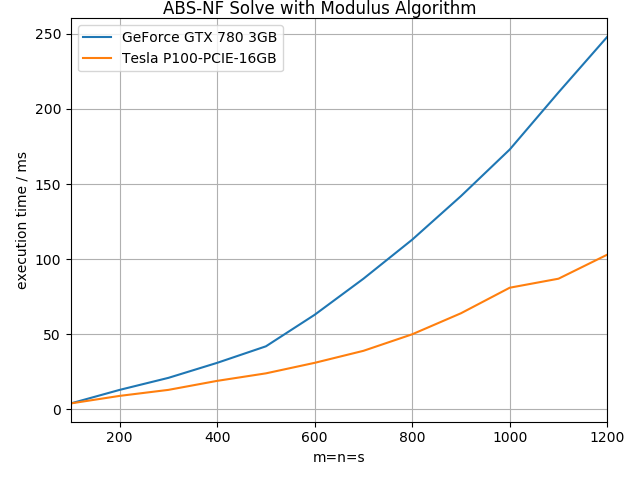
\includegraphics[width=0.6\textwidth]{img/solve_modulus.png}
	\caption{Runtime of the modulus solve implementation}
	\label{fig_modulus_runtime}
\end{figure}

\subsection{Analysis and Notes}
The implementation works correctly and the runtime results in fig. \ref{fig_modulus_runtime} behave as expected. We did not include the runtime of the serial version on purpose. This was for two reasons:
\begin{enumerate}
	\item The numpy implementation calculates the inverse of $J$ directly.
	\item We had to make sure, that each version operates on the exact same data, which we didn't
\end{enumerate}


\end{document}